\documentclass[a4paper]{article}
\usepackage{ctex}
\usepackage{xeCJK}
\usepackage{graphicx}
\usepackage{geometry}
\usepackage{latexsym}
\usepackage{amsmath}
\usepackage{listings}
\lstset{language=Matlab}
\usepackage[framed,numbered,autolinebreaks,useliterate]{mcode}
\usepackage{xcolor}
\usepackage{appendix}
\usepackage{changepage}
\usepackage{algorithm}
\usepackage{algorithmicx}
\usepackage{algpseudocode}  
\usepackage{type1cm}
\usepackage{enumerate}

\makeatletter
\newcommand\dlmu[2][4cm]{\hskip1pt\underline{\hb@xt@ #1{\hss#2\hss}}\hskip3pt}
\makeatother

\title{\Huge Algorithms Analysis and Design}
\author{}
\date{}
\begin{document}

%%封面
\newgeometry{left=2.5cm,right=2.5cm, top=3cm, bottom=3cm}
\thispagestyle{empty}
\begin{figure}[!htbp]
	\centering
	
\includegraphics[width=12cm]{清华校徽.pdf}
\end{figure}
\begin{center}
	{\kaishu \zihao{-0} 算法分析与设计课程作业}\\
	\vspace{0.5cm}
	{\kaishu \zihao{2}  主讲教师:王振波}
\end{center}\vspace{2cm}
\begin{table}[!hbtp]
	\centering
	\LARGE
	\kaishu
	\begin{tabular}{cl}
		\centering
		姓名: & \dlmu[6cm]{冯寅潇}         \\
		学号: & \dlmu[6cm]{2020311833}     \\
		学院: & \dlmu[6cm]{交叉信息研究院} \\
	\end{tabular}
\end{table}

\newgeometry{left=2.5cm,right=2.5cm, top=3cm, bottom=3cm} %%正文页面格式
\maketitle

\section*{Homework 1}
\subsection*{p22, Ex1.1}
\begin{adjustwidth}{1cm}{1cm}
	Decide whether you think the following statement is true or false. If it is true, give a short explanation. If it is false, give a counterexample.
\end{adjustwidth}
\begin{adjustwidth}{2cm}{1cm}
	\emph{True or false? In every instance of the Stable Matching Problem, there is a stable matching containing a pair (m, w) such that m is ranked first on the preference list of w and w is ranked first on the preference list of m.}
\end{adjustwidth}

\subsubsection*{Answer}
False. Counterexample is show blew:
\begin{center}
	\begin{tabular}{|c|c|c|}
		\hline
		Name & Most like                   & Least like                  \\
		\hline
		A    & \textcolor{red}{\textbf{X}} & Y                           \\
		\hline
		B    & \textcolor{red}{\textbf{Y}} & X                           \\
		\hline
		X    & B                           & \textcolor{red}{\textbf{A}} \\
		\hline
		Y    & A                           & \textcolor{red}{\textbf{B}} \\
		\hline
	\end{tabular}
\end{center}
The stable matching is $\{A-X, B-Y\}$. We can see that A and B are not ranked first on the preference list of X and Y. So, it is not necessary to have such pair in stable matching. Actually, there is no such pair at all in this example.
\vspace{2cm}


\subsection*{p22, Ex1.2}
\begin{adjustwidth}{1cm}{1cm}
	Decide whether you think the following statement is true or false. If it is true, give a short explanation. If it is false, give a counterexample.
\end{adjustwidth}
\begin{adjustwidth}{2cm}{1cm}
	\emph{True or false? Consider an instance of the Stable Matching Problem in which there exists a man m and a woman w such that m is ranked first on the preference list of w and w is ranked first on the preference list of m. Then in every stable matching S for this instance, the pair (m, w) belongs to S.}
\end{adjustwidth}

\hspace{2cm}

\subsubsection*{Answer}
True. By contradiction, suppose there exists a stable matching $S$, the adequate pair $(m,w) \notin S$. Assume that $a$ and $b$ are assigned partners of $m$ and $w$ in this matching S. Then, $m$ prefers $w$ to its assigned partner and $w$ prefers $m$ to its assigned partner. So this pair is an unstable pair which contradicts the hypothesis. So, the statement is true.
\vspace{2cm}


\subsection*{p22, Ex1.4}
\begin{adjustwidth}{1cm}{1cm}
	Gale and Shapley published their paper on the Stable Matching Problem in 1962; but a version of their algorithm had already been in use for ten years by the National Resident Matching Program, for the problem of assigning medical residents to hospitals.
	\par Basically, the situation was the following. There were m hospitals, each with a certain number of available positions for hiring residents. There were n medical students graduating in a given year, each interested in joining one of the hospitals. Each hospital had a ranking of the students in order of preference, and each student had a ranking of the hospitals in order of preference. We will assume that there were more students graduating than there were slots available in the m hospitals.
	\par The interest, naturally, was in finding a way of assigning each student to at most one hospital, in such a way that all available positions in all hospitals were filled. (Since we are assuming a surplus of students, there would be some students who do not get assigned to any hospital.)
	\par We say that an assignment of students to hospitals is stable if neither of the following situations arises.
	\begin{itemize}
		\item First type of instability: There are students $s$ and $s'$, and a hospital h, so that \\
		      -  $s$ is assigned to h, and \\
		      -  $s'$ is assigned to no hospital, and \\
		      -  $h$ prefers $s'$ to $s$.
		\item Second type of instability: There are students s and s, and hospitals h and h, so that \\
		      -  $s$ is assigned to $h$, and \\
		      -  $s'$ is assigned to $h'$, and \\
		      -  $h$ prefers $s'$ to $s$, and \\
		      -  $s'$ prefers $h$ to $h'$.
	\end{itemize}
	So we basically have the Stable Matching Problem, except that (i)hospitals generally want more than one resident, and (ii) there is a surplus of medical students.
	\par Show that there is always a stable assignment of students to hospitals,and give an algorithm to find one.
\end{adjustwidth}
\subsubsection*{Answer}
The algorithm is as following aaaaaaafasdfa:
\begin{algorithm}[!htb]
	\caption{Stable assignment algorithm}
	\begin{algorithmic}[1]
		\State Initialize S to empty assignment
		\While{There are hospitals have available positions for hiring residents}
		\State Pick one hospital $h_i$
		\State $h_i$ invites top ranked residents $r_j$ on the ranking list who has not been invites before
		\If{$r_j$ has not been assigned}
		\State add pair $h_i -= r_j$ to matching S
		\ElsIf{$r_j$ prefer $h_i$ to its current assigned hospital $h_k$}
		\State Remove pair  $h_k - r_j$ from matching S
		\State Add pair $h_i -= r_j$ to matching S
		\Else
		\State Invite next resident
		\EndIf
		\EndWhile \\
		\Return Stable assignment S
	\end{algorithmic}
\end{algorithm}
\par For the first type of instability, if $h$ prefers $s'$ to $s$, then, before $s$ is assigned to $h$, $h$ must have invite $s'$. So $s'$ can not been assigned to no hospital.
\par For the second type of instability, If $h$ prefers $s'$ to $s$, then, before $s$ is assigned to $h$, $h$ must have invite $s'$. So the assigned hospital of $s'$ must be higher than $h$ on the ranking list of $s'$. $s'$ can not prefer $h$ to $h'$.
\par In conclusion, The Algorithm above can find the stable assignment.
\vspace{2cm}


\subsection*{p22, Ex1.5}
\begin{adjustwidth}{1cm}{1cm}
	The Stable Matching Problem, as discussed in the text, assumes that all men and women have a fully ordered list of preferences. In this problem we will consider a version of the problem in which men and women can be indifferent between certain options. As before we have a set M of n men and a set W of n women. Assume each man and each woman ranks the members of the opposite gender, but now we allow ties in the ranking. For example (with n = 4), a woman could say that $m_1$ is ranked in first place; second place is a tie between $m_2$ and $m_3$ (she has no preference between them); and $m_4$ is in last place. We will say that $w$ prefers $m$ to $m'$ if m is ranked higher than $m'$ on her preference list (they are not tied).
	\par With indifference in the rankings, there could be two natural notions for stability. And for each, we can ask about the existence of stable matching, as follows.
	\begin{enumerate}[(a)]
		\item A strong instability in a perfect matching S consists of a man m and
		      a woman w, such that each of m and w prefers the other to their partner in S. Does there always exist a perfect matching with no strong instability? Either give an example of a set of men and women with preference lists for which every perfect matching has a strong instability; or give an algorithm that is guaranteed to find a perfect matching with no strong instability.
		\item A weak instability in a perfect matching S consists of a man m and
		      a woman w, such that their partners in S are w and m, respectively,
		      and one of the following holds: \\
		      \quad -  m prefers w to w, and w either prefers m to m or is indifferent
		      between these two choices; or \\
		      \quad -  w prefers m to m, and m either prefers w to w or is indifferent
		      between these two choices. \\
		      In other words, the pairing between m and w is either preferred
		      by both, or preferred by one while the other is indifferent. Does
		      there always exist a perfect matching with no weak instability? Either
		      give an example of a set of men and women with preference lists
		      for which every perfect matching has a weak instability; or give an
		      algorithm that is guaranteed to find a perfect matching with no weak
		      instability.
	\end{enumerate}
\end{adjustwidth}
\subsubsection*{Answer}
\subsubsection*{(a)}
True. The original algorithm is still work. If m prefer w than his assigned partner a, that means m have already proposed to w before m proposed to a. If m have already proposed to w, then the assigned partner of w must be better than m because each change w get a better partner.
\subsubsection*{(b)}
False. Example is show blew:
\begin{center}
	\begin{tabular}{|c|c|c|}
		\hline
		Name & Most like & Least like \\
		\hline
		A    & X         & Y          \\
		\hline
		B    & X         & Y          \\
		\hline
		X    & AB        &            \\
		\hline
		Y    & AB        &            \\
		\hline
	\end{tabular}
\end{center}
\par Wether Y married A or B, another prefer Y than X and Y is indifferent
between A and B. So, there is not such an algorithm guarantee no weak instability

\newpage
\section*{Homework 2}
\subsection*{p68 Ex2.6}
\begin{adjustwidth}{1cm}{1cm}
	Consider the following basic problem. You’re given an array A consisting of n integers $A[1], A[2], . . . , A[n]$. You’d like to output a two-dimensional n-by-n array B in which $B[i, j] (for\quad $i<j$)$ contains the sum of array entries $A[i]$ through $A[j]$—that is, the sum $A[i]+ A[i + 1]+ . . .+ A[j]$. (The value of array entry $B[i, j]$ is left unspecified whenever $i \geq j$, so it doesn’t matter what is output for these values.)
	\par Here’s a simple algorithm to solve this problem.
	\begin{table}[!htbp]
		\centering
		\begin{tabular}{l}
			\hline  %添加表格头部粗线
			For i = 1, 2,..., n                               \\
			\quad For j = i+1, i+2,..., n                     \\
			\qquad Add up array entries $A[i]$ through $A[j]$ \\
			\qquad  Store the result in $B[i,j]$              \\
			\quad Endfor                                      \\
			Endfor                                            \\
			\hline %添加表格底部粗线
		\end{tabular}
	\end{table}

	\begin{enumerate}[(a)]
		\item For some function $f$ that you should choose, give a bound of the
		      form $O(f (n))$ on the running time of this algorithm on an input of
		      size n (i.e., a bound on the number of operations performed by the
		      algorithm).
		\item For this same function f, show that the running time of the algorithm
		      on an input of size n is also $\Omega(f (n))$. (This shows an asymptotically
		      tight bound of $\Theta(f (n))$ on the running time.)
		\item Although the algorithm you analyzed in parts (a) and (b) is the most
		      natural way to solve the problem—after all, it just iterates through
		      the relevant entries of the array B, filling in a value for each—it contains some highly unnecessary sources of inefficiency. Give a different algorithm to solve this problem, with an asymptotically better running time. In other words, you should design an algorithm with running time O(g(n)), where ${\lim_{n \to \infty}\frac{g(n)}{f(n)} = 0}$ .
	\end{enumerate}
\end{adjustwidth}

\subsubsection*{Answer}
\subsubsection*{(a)}
The operation of summation takes no more than n additions. So the upper bound on the number of addition operation performed by the algorithm is no more than $O(n^3)$
\subsubsection*{(b)}
For i from 1 to $\frac{1}{4}n$ and j from $\frac{3}{4}n$ to n, for every $B[i,j]$, it takes at least $\frac{1}{2}n$ additions. Therefor, it takes at least $\frac{1}{4}n*\frac{1}{4}n*\frac{1}{2}n=\frac{1}{32}n^3$ additions. So, the running time of the algorithm  on an input of size n is also $\Omega(n^3)$
\subsubsection*{(c)}
The algorithm is as following:
\begin{algorithm}[!htb]
	\centering
	\caption{Summation matrix algorithm}
	\begin{algorithmic}[1]
		\State Initialize B to all zero matrix
		\For{$i = 1, 2,..., n$}
		\State $B[i,i] = A[i]$
		\For{$j = i+1, i+2,..., n$}
		\State $B[i,j] = B[i,j-1]+A[j]$
		\EndFor
		\EndFor \\
		\Return B
	\end{algorithmic}
\end{algorithm}
\par Each B[i, j] can be calculated by adding once based on B[i, j-1]. So, this algorithm has running time $O(n^2)$
\vspace{2cm}

\subsection*{p69, Ex2.8}
\begin{adjustwidth}{1cm}{1cm}
	You’re doing some stress-testing on various models of glass jars to
	determine the height from which they can be dropped and still not break.
	The setup for this experiment, on a particular type of jar, is as follows.
	You have a ladder with $n$ rungs, and you want to find the highest rung
	from which you can drop a copy of the jar and not have it break. We call
	this the highest safe rung.
	\par It might be natural to try binary search: drop a jar from the middle
	rung, see if it breaks, and then recursively try from rung $n/4$ or $3n/4$
	depending on the outcome. But this has the drawback that you could
	break a lot of jars in finding the answer.
	\par If your primary goal were to conserve jars, on the other hand, you
	could try the following strategy. Start by dropping a jar from the first
	rung, then the second rung, and so forth, climbing one higher each time
	until the jar breaks. In this way, you only need a single jar—at the momentit breaks, you have the correct answer—but you may have to drop it $n$
	times (rather than $log n$ as in the binary search solution).
	\par So here is the trade-off: it seems you can perform fewer drops if
	you’re willing to break more jars. To understand better how this tradeoff
	works at a quantitative level, let’s consider how to run this experiment
	given a fixed “budget” of $k \geq 1$ jars. In other words, you have to determine
	the correct answer—the highest safe rung—and can use at most k jars in
	doing so.
	\begin{enumerate}[(a)]
		\item Suppose you are given a budget of k = 2 jars. Describe a strategy for
		      finding the highest safe rung that requires you to drop a jar at most
		      $f(n)$ times, for some function $f(n)$ that grows slower than linearly. (In
		      other words, it should be the case that $lim_{n→∞} f(n)/n = 0$.)
		\item Now suppose you have a budget of k > 2 jars, for some given k.
		      Describe a strategy for finding the highest safe rung using at most
		      k jars. If $f_k(n)$ denotes the number of times you need to drop a jar
		      according to your strategy, then the functions $f_1, f_2, f_3, . . .$ should have the property that each grows asymptotically slower than the previous
		      one: $lim_{n→∞} f_k(n)/f_{k−1}(n) = 0$ for each k.
	\end{enumerate}
\end{adjustwidth}

\subsubsection*{Answer}
\subsubsection*{(a)}
The algorithm is as following:
\begin{algorithm}[!htb]
	\caption{Algorithm of Ex2.8(a)}
	\begin{algorithmic}[1]
		\State Divide $n$ rungs into $\sqrt{n}$ parts. Each part has $\sqrt{n}$ rungs.
		\State Start by dropping the first jar from the highest rung of the first rung part.
		\Repeat \\
		\quad Climbing $\sqrt{n}$ rungs higher to the highest rung of the next part.
		\Until \\
		\quad The glass jar breaks
		\State Start by dropping the second jar from the first rung of the  part in which the first jar has broken.
		\Repeat \\
		\quad Climbing one rung higher each time
		\Until\\
		\quad The glass jar breaks\\
		\Return{The height}
	\end{algorithmic}
\end{algorithm}
\par It takes at most $2\sqrt{n}$ times test to determine the height. So, this algorithm has running time $O(\sqrt{n})$
\vspace{1cm}

\subsubsection*{(b)}
The algorithm is as following:
\begin{algorithm}[!htb]
	\caption{Algorithm of Ex2.8(b)}
	\begin{algorithmic}[1]
		\State Divide $n$ rungs into $n^{\frac{1}{k}}$ parts. Each part has $n^{\frac{k-1}{k}}$ rungs. Then, divide every part into $n^{\frac{1}{k}}$ smaller parts and so on. We totally have
		\For{$i = 1, 2,..., k-1$}
		\State Start by dropping the $i^{th}$ jar from the highest rung of the first rung part in this level of partition.
		\Repeat \\
		\qquad Climbing $n^\frac{k-i}{k}$ rungs higher to the highest rung of the next part in this level of partition.
		\Until \\
		\qquad The glass jar breaks
		\State Do tests in this part in which last jar has broken by next level of partition.
		\EndFor
		\State Start by dropping the $k^{th}$ jar from the first rung of the part of this level, in which last jar has broken.
		\Repeat \\
		\quad Climbing one rung higher each time
		\Until\\
		\quad The glass jar breaks\\
		\Return{The height}
	\end{algorithmic}
\end{algorithm}
\par For a given k, it takes $O(kn^{\frac{1}{k}})$ times test to determine the height. So,
$$lim_{n→∞} f_k(n)/f_{k−1}(n) = lim_{n→∞} \frac{kn^{\frac{1}{k}}}{(k-1)n^{\frac{1}{k-1}}} = 0 $$
\vspace{2cm}

\subsection*{p107 Ex3.5}
\begin{adjustwidth}{1cm}{1cm}
	A binary tree is a rooted tree in which each node has at most two children.
	Show by induction that in any binary tree the number of nodes with two
	children is exactly one less than the number of leaves.
\end{adjustwidth}

\subsubsection*{Answer}
Suppose T is a binary tree with $n_1$ nodes with one child, $n_2$ nodes with two children and $m$ leaves without child. There are two ways to add a node.
\begin{itemize}
	\item Add a leaf to a leaf node. Then, the new tree will have $n_1+1$ nodes with one child $n_2$ nodes with two children and $m-1+1 = m$ leaves without child.
	\item Add a leaf to a node with one child. Then, the new tree will have $n_1-1$ nodes with one child $n_2+1$ nodes with two children and $m+1$ leaves without child.
\end{itemize}
\par That means adding node will increase the number of $n_2$ and $m$ simultaneously. For the simplest tree which only have one root node, $n_2 = 0$, $m = 1$, And every binary tree can be built from root node by adding nodes one by one. So, in any binary tree the number of nodes with two
children is exactly one less than the number of leaves.
\vspace{2cm}

\subsection*{p107 Ex3.6}
\begin{adjustwidth}{1cm}{1cm}
	We have a connected graph $G = (V, E)$, and a specific vertex $u \in V$. Suppose
	we compute a depth-first search tree rooted at u, and obtain a tree T that
	includes all nodes of G. Suppose we then compute a breadth-first search
	tree rooted at u, and obtain the same tree T. Prove that $G = T$. (In other
	words, if T is both a depth-first search tree and a breadth-first search
	tree rooted at u, then G cannot contain any edges that do not belong to
	T.)
\end{adjustwidth}

\subsubsection*{Answer}
By contradiction, suppose there exists an edge $e=\{A-B\} \in G$ but $e=\{A-B\}\notin T$. As T is a tree, so there must be a path $\{A-C-B\}$ from A to B. C is a vertex different from A and B. According to the distance between A, B, C and the root u in T, there are two conditions:
\begin{itemize}
	\item $d_T(A,u),d_T(B,u) > d_T(C,u) $. Then, C is the parent node of both A and B. In the process of constructing DFS tree, after C has been added to T, no matter A or B is added to T first, $\{A-B\}\in T$.
	\item $d_T(A,u) > d_T(C,u) > d_T(B,u)$(or  $d_T(B,u) > d_T(C,u) > d_T(A,u)$). Then, B is the parent node of both A and C. In the process of constructing BFS tree, after B has been added to T, as C haven't been added to T, A will be added to T after B. then, $\{A-B\}\in T$
\end{itemize}
\par In conclusion, $G = T$.

\newpage
\section*{Homework 3}
\subsection*{p107 Ex3.2}
\begin{adjustwidth}{1cm}{1cm}
	The algorithm described in Section 3.6 for computing a topological ordering
	of a DAG repeatedly finds a node with no incoming edges and deletes
	it. This will eventually produce a topological ordering, provided that the
	input graph really is a DAG.
	\par But suppose that we’re given an arbitrary graph that may or may not
	be a DAG. Extend the topological ordering algorithm so that, given an
	input directed graph G, it outputs one of two things: (a) a topological
	ordering, thus establishing that G is a DAG; or (b) a cycle in G, thus
	establishing that G is not a DAG. The running time of your algorithm
	should be $O(m + n)$ for a directed graph with n nodes and m edges.
\end{adjustwidth}

\subsubsection*{Answer}
The Algorithm is on the next page
\begin{algorithm}[!htb]
	\caption{Algorithm of Ex3.2}
	\begin{algorithmic}[1]
		\State Initialize empty ordering $O$ and empty circle $C$
		\While{There is a node $v \in G$ with no incoming edge}
		\State Add the node $v$ into $O$.
		\State Delete v and connected edges from $G$ and get new $G = G-\{v\}$
		\EndWhile
		\If{$G == \emptyset$}\\
		\Return{The topological ordering $O$}
		\Else
		\State Mark all nodes as unreached
		\State Apply DFS Search from any node $v$
		\Function{DFS}{G,v}
		\State Mark $v$ as being reaching
		\If{There is a path from $v$ to an being reaching node $u \in G$}
		\State There is a circle $u \rightarrow v \rightarrow u$
		\State Add $u$ to the end of circle $C$
		\State Return\{Circle is found\}
		\EndIf
		\While{There is a path from $v$ to an unreached node $u \in G$}
		\State Apply DFS to node $u$: (DFS(G,u))
		\If{Return "Circle is found"}
		\State Add $u$ to the end of circle $C$
		\State Return\{Circle is found\}
		\EndIf
		\EndWhile
		\State Mark $v$ as reached
		\State Return
		\EndFunction
		\EndIf\\
		\Return{The Circle $C$}
	\end{algorithmic}
\end{algorithm}

\par Topological ordering is $O(m+n)$ and DFS search is $O(m+n)$. So, the extend algorithm is $O(m+n)$

\vspace{2cm}



\subsection*{p109 Ex3.8}
\begin{adjustwidth}{1cm}{1cm}
	A number of stories in the press about the structure of the Internet and
	the Web have focused on some version of the following question: How
	far apart are typical nodes in these networks? If you read these stories
	carefully, you find that many of them are confused about the difference
	between the diameter of a network and the average distance in a network;
	they often jump back and forth between these concepts as though they’re
	the same thing.
	\par As in the text, we say that the distance between two nodes u and v
	in a graph G = (V, E) is the minimum number of edges in a path joining
	them; we’ll denote this by dist(u, v). We say that the diameter of G is
	the maximum distance between any pair of nodes; and we’ll denote this
	quantity by diam(G).
	\par Let’s define a related quantity, which we’ll call the average pairwise
	distance in G (denoted apd(G)). We define apd(G) to be the average, over
	all $\left(\begin{array}{l}n \\ 2\end{array}\right)$ sets of two distinct nodes u and v, of the distance between u and v.
	That is, \\
	$$\operatorname{apd}(G)=\left[\sum_{\{u, v\} \subseteq V} \operatorname{dist}(u, v)\right] /\left(\begin{array}{l}n\\2\end{array}\right)$$
	while
	$$\operatorname{apd}(G)=[\operatorname{dist}(u, v)+\operatorname{dist}(u, w)+\operatorname{dist}(v, w)] / 3=4 / 3$$
	\par Of course, these two numbers aren’t all that far apart in the case of
	this three-node graph, and so it’s natural to ask whether there’s always a
	close relation between them. Here’s a claim that tries to make this precise.\\
	\par \emph{Claim: There exists a positive natural number c so that for all connected graphs
		G, it is the case that}
	$$\frac{\operatorname{diam}(G)}{\operatorname{apd}(G)} \leq c$$
	Decide whether you think the claim is true or false, and give a proof of
	either the claim or its negation.
\end{adjustwidth}

\subsubsection*{Answer}
False. Counterexample is described below:
\par There is a path in G from $v_1$ to $v_{\sqrt{n}}$ connected $\sqrt{n}$ nodes; Other $n-\sqrt{n}$ nodes are connected to $v_1$. $diam(G)$ is $O(\sqrt{n})$, $\sum_{\{u, v\} \subseteq V} \operatorname{dist}(u, v)$ is $O(n^2)$, $\left(\begin{array}{l}n \\ 2\end{array}\right)$ is $O(n^2)$, so, $apd(G)$ is $O(1)$. As $n \rightarrow \infty$, $\frac{\operatorname{diam}(G)}{\operatorname{apd}(G)} \rightarrow \infty$
\vspace{2cm}

\subsection*{p190 Ex4.4}
\begin{adjustwidth}{1cm}{1cm}
	Some of your friends have gotten into the burgeoning field of time-series
	data mining, in which one looks for patterns in sequences of events that
	occur over time. Purchases at stock exchanges—what’s being bought—
	are one source of data with a natural ordering in time. Given a long
	sequence $S$ of such events, your friends want an efficient way to detect
	certain “patterns” in them—for example, they may want to know if the
	four events
	\par \emph{buy Yahoo, buy eBay, buy Yahoo, buy Oracle}\\
	occur in this sequence $S$, in order but not necessarily consecutively.
	\par They begin with a collection of possible events (e.g., the possible
	transactions) and a sequence S of n of these events. A given event may
	occur multiple times in $S$ (e.g., Yahoo stock may be bought many times
	in a single sequence $S$). We will say that a sequence $S'$ is a subsequence
	of $S$ if there is a way to delete certain of the events from S so that the
	remaining events, in order, are equal to the sequence $S'$. So, for example,
	the sequence of four events above is a subsequence of the sequence
	\par \emph{buy Amazon, buy Yahoo, buy eBay, buy Yahoo, buy Yahoo,
		buy Oracle}
	\par Their goal is to be able to dream up short sequences and quickly
	detect whether they are subsequences of $S$. So this is the problem they
	pose to you: Give an algorithm that takes two sequences of events—$S'$ of
	length m and $S$ of length n, each possibly containing an event more than
	once—and decides in time $O(m + n)$ whether $S'$ is a subsequence of S.
\end{adjustwidth}
\subsubsection*{Answer}
The Algorithm is as following:
\begin{algorithm}[!htb]
	\caption{Algorithm of Ex4.4}
	\begin{algorithmic}[1]
		\State Initialize pointer at location 0 of S
		\For{$i \in S'$}
		\If{next events $j$ appear in $S$ after pointer}
		\State Change pointer to the location of $j$
		\Else
		\State Return False
		\EndIf
		\EndFor\\
		\Return{True}
	\end{algorithmic}
\end{algorithm}
\par We can know the result after the pointer traversing the entire sequence. So, the algorithm is  $O(m + n)$.

\vspace{2cm}



\subsection*{p191 Ex4.6}
\begin{adjustwidth}{1cm}{1cm}
	Your friend is working as a camp counselor, and he is in charge of
	organizing activities for a set of junior-high-school-age campers. One of
	his plans is the following mini-triathalon exercise: each contestant must
	swim 20 laps of a pool, then bike 10 miles, then run 3 miles. The plan is
	to send the contestants out in a staggered fashion, via the following rule:
	the contestants must use the pool one at a time. In other words, first one
	contestant swims the 20 laps, gets out, and starts biking. As soon as this
	first person is out of the pool, a second contestant begins swimming the
	20 laps; as soon as he or she is out and starts biking, a third contestant
	begins swimming . . . and so on.)
	Each contestant has a projected swimming time (the expected time it
	will take him or her to complete the 20 laps), a projected biking time (the
	expected time it will take him or her to complete the 10 miles of bicycling),
	and a projected running time (the time it will take him or her to complete
	the 3 miles of running). Your friend wants to decide on a schedule for the
	triathalon: an order in which to sequence the starts of the contestants.
	Let’s say that the completion time of a schedule is the earliest time at
	which all contestants will be finished with all three legs of the triathalon,
	assuming they each spend exactly their projected swimming, biking, and
	running times on the three parts. (Again, note that participants can bike
	and run simultaneously, but at most one person can be in the pool at
	any time.) What’s the best order for sending people out, if one wants the
	whole competition to be over as early as possible? More precisely, give
	an efficient algorithm that produces a schedule whose completion time
	is as small as possible.

\end{adjustwidth}

\subsubsection*{Answer}
The strategy is letting contestant who takes longer time for biking and 3 miles begin to swim earlier in the schedule sequence. We can approve this is the optimal algorithm by using contradiction:
\par Suppose A takes longer time for biking and 3 miles than B, but is after B in the schedule sequence. Without loss of generality, let's assume A is next to B. Suppoese A and B take $t1_A, t1_B, t2_A, t2_B, t3_A, t3_B$ for swimming, biking and 3 miles. It takes $t1_B + t1_A + t2_A + t3_A$ for them to finish. However, if We let A swim before B,it takes $t1_A + maximum\{(t2_A+t3_A), (t1_B+t2_B+t3_B)\}$
\begin{equation}
	\begin{aligned}
		t_{sum} & = t1_A + maximum\{(t2_A+t3_A), (t1_B+t2_B+t3_B)\}    \\
		        & \leq t1_A + maximum\{(t2_A+t3_A), (t1_B+t2_A+t3_A)\} \\
		        & \leq t1_B + t1_A + t2_A + t3_A
	\end{aligned}
\end{equation}
\par So, the algorithm is optimal.

\newpage
\section*{Homework 4}
\subsection*{p192 Ex4.8}
\begin{adjustwidth}{1cm}{1cm}
	Suppose you are given a connected graph G, with edge costs that are all
	distinct. Prove that G has a unique minimum spanning tree.
\end{adjustwidth}

\subsubsection*{Answer}
By contradiction, suppose $T$ and $T'$ are two distinct minimum spanning trees of G. There must be an edge $e \in T', e\notin T$, If we add e to $T$, a circle will be formed. If e is not the most expensive edge, it is condradicting the fact that $T$ is a MST. If e is the most expensive edge, there exists an edge $e'\in T, e'\notin T'$ in the circle. If we add $e'$ to $T'$, a circle contain $e$ and $e'$ will be formed. it is condradicting the fact that $T'$ is a MST.
\vspace{2cm}


\subsection*{p197 Ex4.18}
\begin{adjustwidth}{1cm}{1cm}
	Your friends are planning an expedition to a small town deep in the Canadian
	north next winter break. They've researched all the travel options
	and have drawn up a directed graph whose nodes represent intermediate
	destinations and edges represent the roads between them.
	\par In the course of this, they've also learned that extreme weather causes
	roads in this part of the world to become quite slow in the winter and
	may cause large travel delays. They’ve found an excellent travel Web site
	that can accurately predict how fast they’ll be able to travel along the
	roads; however, the speed of travel depends on the time of year. More
	precisely, the Web site answers queries of the following form: given an
	edge $e = (v, w)$ connecting two sites v and w, and given a proposed starting
	time t from location v, the site will return a value $f_e(t)$, the predicted
	arrival time at w. The Web site guarantees that $f_e(t)\geq t$ for all edges e
	and all times t (you can’t travel backward in time), and that $f_e(t)$ is a
	monotone increasing function of t (that is, you do not arrive earlier by
	starting later). Other than that, the functions $f_e(t)$ may be arbitrary. For
	example, in areas where the travel time does not vary with the season,
	we would have $f_e(t) = t + l_e$, where $l_e$ is the time needed to travel from the
	beginning to the end of edge e.
	\par Your friends want to use the Web site to determine the fastest way
	to travel through the directed graph from their starting point to their
	intended destination. (You should assume that they start at time 0, and
	that all predictions made by the Web site are completely correct.) Give a
	polynomial-time algorithm to do this, where we treat a single query to
	the Web site (based on a specific edge e and a time t) as taking a single
	computational step.
\end{adjustwidth}
\subsubsection*{Answer}
The Algorithm is as following:
\begin{algorithm}[!htb]
	\caption{Algorithm of Ex4.18}
	\begin{algorithmic}[1]
		\State Initialize explored nodes set $S = {s}$, earliest arrival time of s $d(s)=0$ and last node of s $r(s) = \emptyset$
		\While{$S \neq V$}
		\State Compute the distances from nodes inside S to nodes outside S and have a direct edge. Each distance $d_{ab}$is decided by $a, b$ and the distace from $a$ to $s$
		\State Find the shortest distance $d_{ab}$, add b to S and define $d(b)=d_a+d_{ab}$ $r(b)=a$
		\EndWhile\\
		\Return
	\end{algorithmic}
\end{algorithm}
\par The Correctness is guaranteed because that $f_e(t)$ is a
monotone increasing function of t. For any path from a to b, earlier reach to a, earlier reach to b. The algorithm above computer the earliest arrival time one node by one node.
\par Similar to DijKstra's algorithm. This algorithm is $O(mlogn)$
\vspace{2cm}


\subsection*{p246 Ex5.1}
\begin{adjustwidth}{1cm}{1cm}
	You are interested in analyzing some hard-to-obtain data from two separate
	databases. Each database contains n numerical values—so there are
	2n values total—and you may assume that no two values are the same.
	You’d like to determine the median of this set of 2n values, which we will
	define here to be the $n_{th}$ smallest value.
	\par However, the only way you can access these values is through queries
	to the databases. In a single query, you can specify a value k to one of the
	two databases, and the chosen database will return the kth smallest value
	that it contains. Since queries are expensive, you would like to compute
	the median using as few queries as possible.
	Give an algorithm that finds the median value using at most $O(log n)$
	queries.
\end{adjustwidth}
\subsubsection*{Answer}
First, we can compare the median of the two database. If $A[\lfloor \frac{n}{2} \rfloor]<B[\lfloor \frac{n}{2} \rfloor]$, we can know the median number is on higher position of A and lower position of B. So we can reduce half number of the two databse.
\par The Algorithm is as following, evaluate MEDIAN(A[n],B[n],n):
\begin{algorithm}[!htb]
	\caption{Algorithm of Ex5.1}
	\begin{algorithmic}[1]
		\Function{median}{a[n],b[n],k}
		\If{k==1}
		\State Return $min\{a[1],b[1]\}$
		\ElsIf{$a[\lfloor \frac{k}{2} \rfloor] < b[\lfloor \frac{k}{2} \rfloor]$}
		\State Return MEDIAN(a[$\lfloor \frac{k}{2} \rfloor$:n], b[1:$\lfloor \frac{k}{2} \rfloor$],$\lceil \frac{k}{2} \rceil$)
		\Else
		\State Return MEDIAN(a[1:$\lfloor \frac{k}{2} \rfloor$], b[$\lfloor \frac{k}{2} \rfloor$:n],$\lceil \frac{k}{2} \rceil$)
		\EndIf
		\EndFunction
	\end{algorithmic}
\end{algorithm}
\par For each iteration, each database is queried once. It will iterate for a maximum of $\lceil log_2n \rceil$ times. So, the algorithm is $O(logn)$.
\vspace{2cm}

\subsection*{p246 Ex5.2}
\begin{adjustwidth}{1cm}{1cm}
	Recall the problem of finding the number of inversions. As in the text,
	we are given a sequence of n numbers $a_1, . . . , a_n$, which we assume are all
	distinct, and we define an inversion to be a pair $i < j$ such that $a_i > a_j$.
	\par We motivated the problem of counting inversions as a good measure
	of how different two orderings are. However, one might feel that this
	measure is too sensitive. Let’s call a pair a significant inversion if $i < j$ and
	$a_i > 2a_j$. Give an $O(n log n)$ algorithm to count the number of significant
	inversions between two orderings.
\end{adjustwidth}

\subsubsection*{Answer}
The Algorithm is as following, evaluate INVERSION(a[n]):
\begin{algorithm}[!htb]
	\caption{Algorithm of Ex5.2}
	\begin{algorithmic}[1]
		\Function{inversion}{a[n]}
		\If{n==1} Return 0
		\Else
		\State x = $a[1:\lfloor \frac{n}{2} \rfloor]$; y = $a[\lceil \frac{n}{2} \rceil:n]$
		\State Initialize pointers i and j at the first index of x and y; counter=0;
		\While{i,j are not at end of x and y}
		\If{$a_i>2a_j$}
		\State counter = counter + $\lfloor \frac{n}{2} \rfloor - i + 1$; j++
		\Else
		\State i++
		\EndIf
		\EndWhile
		\State Return INVERSION(x)+INVERSION(y)+counter
		\EndIf
		\EndFunction
	\end{algorithmic}
\end{algorithm}
\par The algorithm is $O(n log n)$.


\newpage
\section*{Homework 5}
\subsection*{Prove the Master Theorem}
\begin{adjustwidth}{1cm}{1cm}
	Suppose that $T(n)$ is a function on the nonnegative integers that satisfies the recurrence
	$$
		T(n)=a T\left(\frac{n}{b}\right)+f(n)
	$$
	where $\frac{n}{b}$ means either $\lfloor n / b\rfloor$ or $\lceil n / b\rceil .$ Let $k=\log _{b} a,$
	\begin{itemize}
		\item Case 1. If $f(n)=O\left(n^{k-\epsilon}\right)$ for some constant $\epsilon>0$, then $T(n)=\Theta\left(n^{k}\right)$
		\item Case 2. If $f(n)=\Theta\left(n^{k} \log ^{p} n\right)$, then $T(n)=\Theta\left(n^{k} \log ^{p+1} n\right)$
		\item Case 3. If $f(n)=\Omega\left(n^{k+\epsilon}\right)$ for some constant $\epsilon>0$ and if $a f(n / b) \leq c f(n)$ for some constant $c<1$ and all sufficiently large $n$, then $T(n)=\Theta(f(n))$
	\end{itemize}
\end{adjustwidth}

\subsubsection*{Answer}
By mathematical induction, all the three cases are valid for $n=2$. Suppose they are valid for $n = m$.
\begin{itemize}
	\item Case 1. If $f(n)=O\left(n^{k-\epsilon}\right)$, $T(n)=\Theta\left(n^{k}\right)$,
	      $$T(bm)=a T\left(m\right)+f(bm)=b^k\Theta\left(m^{k}\right)+O\left((bm))^{k-\epsilon}\right)=\Theta\left((bm)^{k}\right)$$
	\item Case 2. If $f(n)=\Theta\left(n^{k} \log ^{p} n\right)$, $T(n)=\Theta\left(n^{k} \log ^{p+1} n\right)$,
	      $$
		      T(bm)=b^k\Theta\left(m^{k} \log ^{p+1} m\right)+\Theta\left((bm)^{k} \log ^{p} bm\right)
	      $$
	      $$
		      =\Theta\left((bm)^{k} (log^{p+1}m + \log ^{p} bm)\right)=\Theta\left((bm)^{k} \log ^{p+1} bm\right)
	      $$
	\item If $f(n)=\Omega\left(n^{k+\epsilon}\right)$ for some constant $\epsilon>0$, $a f(n / b) \leq c f(n)$ for some constant $c<1$ and all sufficiently large $n$ and if $T(n)=\Theta(f(n))$,
	      $$
		      T(bm)=b^k\Omega\left(m^{k+\epsilon}\right)+\Theta(\Omega\left((bm)^{k+\epsilon}\right)) \leq c\Omega\left(m^{k+\epsilon}\right) + \Theta(\Omega\left((bm)^{k+\epsilon}\right))
	      $$
	      so, $T(bm) = \Theta(f(bm))$
\end{itemize}

So far, we have already proved the condition of $n=b^k$. For any other integer, we can always extend it to $n=b^k$ without affecting the time complexity.
\vspace{2cm}

\subsection*{p246 Ex5.3}
\begin{adjustwidth}{1cm}{1cm}
	Suppose you're consulting for a bank that's concerned about fraud detection, and they come to you with the following problem. They have a collection of $n$ bank cards that they've confiscated, suspecting them of being used in fraud. Each bank card is a small plastic object, containing a magnetic stripe with some encrypted data, and it corresponds to a unique account in the bank. Each account can have many bank cardscorresponding to it, and we'll say that two bank cards are equivalent if they correspond to the same account.

	It's very difficult to read the account number off a bank card directly, but the bank has a high-tech "equivalence tester" that takes two bank cards and, after performing some computations, determines whether they are equivalent.

	Their question is the following: among the collection of $n$ cards, is there a set of more than $n / 2$ of them that are all equivalent to one another? Assume that the only feasible operations you can do with the cards are to pick two of them and plug them in to the equivalence tester. Show how
	to decide the answer to their question with only $O(n \log n)$ invocations of the equivalence tester.
\end{adjustwidth}

\subsubsection*{Answer}
\par The Algorithm is as following:
\begin{algorithm}[!htb]
	\caption{Algorithm of Ex5.3}
	\begin{algorithmic}[1]
		\Function{F}{$n$ cards}
		\If{n==1}
		\State Return{This card}
		\ElsIf{F(Half of these n cards) or F(The other half of these n cards) $\neq$ NONE}
		\State Test any of the returned m casds with all the cards in the other half.
		\If{There are more than $n/2-m$ equivalent cards in the other half}
		\State Return $m'$ equivalent cards
		\EndIf
		\Else
		\State Return NONE
		\EndIf
		\EndFunction
	\end{algorithmic}
\end{algorithm}
\par The algorithm is $O(logn)$.
\vspace{2cm}


\subsection*{p247 Ex5.4}
\begin{adjustwidth}{1cm}{1cm}
	You've been working with some physicists who need to study, as part of their experimental design, the interactions among large numbers of very small charged particles. Basically, their setup works as follows. They have an inert lattice structure, and they use this for placing charged particles at regular spacing along a straight line. Thus we can model their structure as consisting of the points $\{1,2,3, \ldots, n\}$ on the real line; and at each of these points $j,$ they have a particle with charge $q_{j} .$ (Each charge can be either positive or negative.)

	They want to study the total force on each particle, by measuring it and then comparing it to a computational prediction. This computational part is where they need your help. The total net force on particle $j,$ by Coulomb's Law, is equal to
	$$
		F_{j}=\sum_{i<j} \frac{C q_{i} q_{j}}{(j-i)^{2}}-\sum_{i>j} \frac{C q_{i} q_{j}}{(j-i)^{2}}
	$$
	They've written the following simple program to compute $F_{j}$ for all $j$
	\begin{figure}[!htbp]
		\centering
		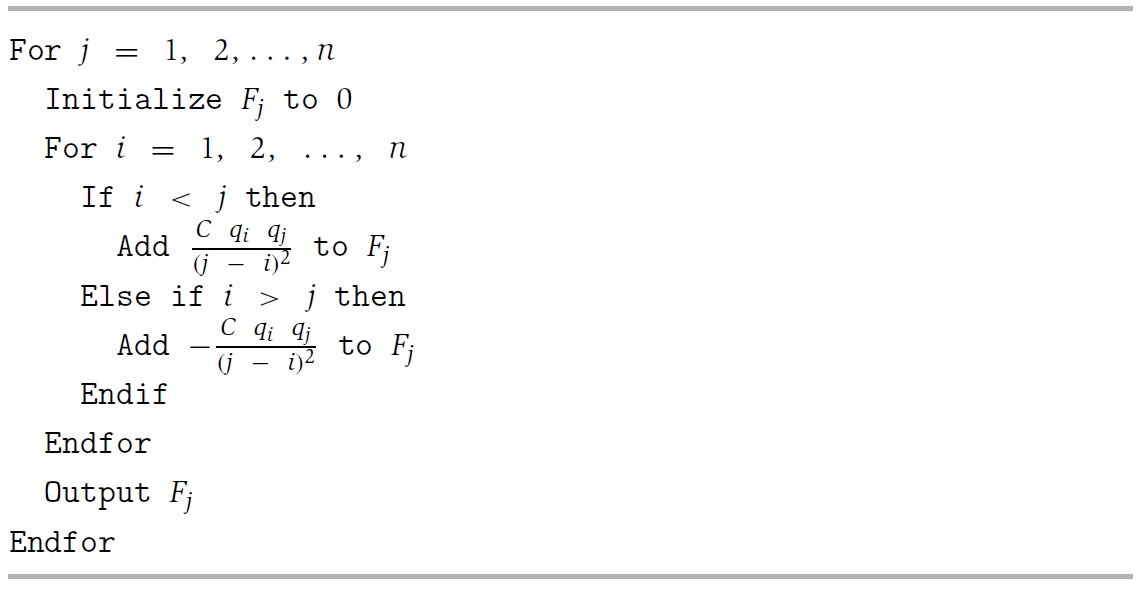
\includegraphics[width=12cm]{Pictures/EX5.4.png}
	\end{figure}

	The trouble is, for the large values of $n$ they're working with, the program takes several minutes to run. On the other hand, their experimental setup is optimized so that they can throw down $n$ particles, perform the measurements, and be ready to handle $n$ more particles within a few seconds. So they'd really like it if there were a way to compute all the forces $F_{j}$ much more quickly, so as to keep up with the rate of the experiment.
	Help them out by designing an algorithm that computes all the forces $F_{j}$ in $O(n \log n)$ time.
\end{adjustwidth}

\subsubsection*{Answer}
We can first construct a vector $\vec{a}=\left(\frac{1}{n^2}, \ldots, \frac{1}{4},1,0,-1,-\frac{1}{4},\ldots -\frac{1}{n^2}\right)$. It takes $O(n)$ time. Assume $\vec{q} = (q_1,q_2,\ldots, q_n). $Then we can use FFT to compute the convolution of $\vec{a}\otimes \vec{q}$. The total time is $O(nlogn)$.
\vspace{2cm}

\newpage
\section*{Homework 6}
\subsection*{p248 Ex5.5}
\begin{adjustwidth}{1cm}{1cm}
	Hidden surface removal is a problem in computer graphics that scarcely needs an introduction: when Woody is standing in front of Buzz, you should be able to see Woody but not Buzz; when Buzz is standing in front of Woody, . . . well, you get the idea.

	The magic of hidden surface removal is that you can often compute things faster than your intuition suggests. Here's a clean geometric example to illustrate a basic speed-up that can be achieved. You are given $n$ nonvertical lines in the plane, labeled $L_{1}, \ldots, L_{n},$ with the $t^{\mathrm{h}}$ line specified by the equation $y=a_{i} x+b_{i} .$ We will make the assumption that no three of the lines all meet at a single point. We say line $L_{i}$ is uppermost at a given $x$ -coordinate $x_{0}$ if its $y$ -coordinate at $x_{0}$ is greater than the $y$ -coordinates of all the other lines at $x_{0}: a_{i} x_{0}+b_{i}>a_{j} x_{0}+b_{j}$ for all $j \neq i .$ We say line $L_{i}$ is visible if there is some $x$ -coordinate at which it is uppermost-intuitively, some portion of it can be seen if you look down from " $y=\infty$."

	Give an algorithm that takes $n$ lines as input and in $O(n \log n)$ time returns all of the ones that are visible. Figure 5.10 gives an example.
\end{adjustwidth}
\subsubsection*{Answer}
The Algorithm is as following:
\begin{algorithm}[!htb]
	\caption{Algorithm of Ex5.5}
	\begin{algorithmic}[1]
		\State Sort all lines by slope
		\Function{F}{$n$ ordered lines}
		\If{n==2}
		\State Return{ The intersection and two line}
		\Else
		\State L1 = F(The first half of these n lines)
		\State L2 = F(The other half of these n lines)
		\State Slope of lines in L1 is always smaller than slope of lines in L2
		\State L1 and L2 are two broken line with p-1 intersection points, p segments and q-1 intersection points, q segments. As the x coordinate of these p-1 and q-1 intersection points are in order, it takes no more than O(p+q) time to find the intersection point k of these two broken line.
		\State After we have found k, lines(segments) in L1 with smaller endpoint(intersection point) x coordinate are visible;  lines(segments) in L2 with larger endpoint(intersection point) x coordinate are visible.
		\State Return{ Visible lines and intersection points in order}
		\EndIf
		\EndFunction
	\end{algorithmic}
\end{algorithm}
\par $p+q$ is always smaller than n, so the Algorithm is $O(nlogn)$
\vspace{2cm}

\subsection*{p248 Ex5.6}
\begin{adjustwidth}{1cm}{1cm}
	Consider an $n$ -node complete binary tree $T,$ where $n=2^{d}-1$ for some $d$. Each node $v$ of $T$ is labeled with a real number $x_{v}$. You may assume that the real numbers labeling the nodes are all distinct. A node $v$ of $T$ is a local minimum if the label $x_{v}$ is less than the label $x_{w}$ for all nodes $w$ that are joined to $v$ by an edge.

	You are given such a complete binary tree $T$, but the labeling is only specified in the following implicit way: for each node $v$, you can determine the value $x_{v}$ by probing the node $v .$ Show how to find a local minimum of $T$ using only $O(\log n)$ probes to the nodes of $T$.
\end{adjustwidth}

\subsubsection*{Answer}
We probe node from root. If the two son is bigger, than the root is the local minimum. Otherwise, if the one of the two son is smaller, we choose any smaller son and repeat the above. As each time we choose a son node smaller than the parent, we stop at a local minimum, or we stop at a leaf node. The leaf node is also satisfied the definition of local minimum. The algorithm is abviously $O(logn)$.
\vspace{2cm}


\subsection*{p317 Ex6.6}
\subsubsection*{Answer}
The Algorithm is as following:
\begin{algorithm}[!htb]
	\caption{Algorithm of Ex6.6}
	\begin{algorithmic}[1]
		\Function{F}{first $n$ words}
		\If{n==0}
		\State Return{ 0}
		\Else
		\For{i = 1 to n}
		\State F($i$) = $\infty$
		\For{j = 1 to i}
		\If{$\left[\sum_{i=j}^{n-1}\left(c_{i}+1\right)\right]+c_{n} \leq L$}
		\State $slack(j,n) = L-\left[\sum_{i=j}^{n-1}\left(c_{i}+1\right)\right]-c_{n}$
		\Else
		\State slack(j,n) = $\infty$
		\EndIf
		\If{$slack(j,n)$+F(first $j-1$ words) < F($i$)}
		\State F($i$) = $slack(j,n)$+F(first $j-1$ words)
		\EndIf
		\EndFor
		\EndFor
		\EndIf \\
		\Return F(n)
		\EndFunction
	\end{algorithmic}
\end{algorithm}
\par $p+q$ is always smaller than n, so the Algorithm is $O(nlogn)$
\vspace{2cm}



\subsection*{p319 Ex6.8}
\subsubsection*{Answer}
\subsubsection*{(a)}
False. Example is show blew:
\begin{center}
	\begin{tabular}{ccccc}
		\hline
		i      & 1 & 2  & 3  & 4 \\
		\hline
		$x_i$  & 1 & 10 & 10 & 2 \\
		\hline
		$f(i)$ & 1 & 2  & 4  & 8 \\
		\hline
	\end{tabular}
\end{center}
\par The algorithm in (a) will return 4. However, the correct answer is a total of 5.

\subsubsection*{(b)}
The Algorithm is as following:
\begin{algorithm}[!htb]
	\caption{Algorithm of Ex6.8}
	\begin{algorithmic}[1]
		\Function{F}{$n$}
		\If{n==0}
		\State Return{ 0}
		\Else
		\For{i = 1 to n}
		\State F($i$) = 0
		\For{j = 0 to i}
		\State s(j,i) = $min\{\min \left(x_{i}, f(j)\right)\}$
		\If{$s(j,i)$+F(j) > F($i$)}
		\State F($i$) = $s(j,i)$+F(j)
		\EndIf
		\EndFor
		\EndFor
		\EndIf
		\EndFunction
	\end{algorithmic}
\end{algorithm}


\newpage
\section*{Homework 7}
\subsection*{p328 Ex6.18}
\begin{adjustwidth}{1cm}{1cm}
	Consider the sequence alignment problem over a four-letter alphabet $\left(z_{1}, z_{2}, z_{3}, z_{4}\right),$ with a given gap cost and given mismatch costs. Assume that each of these parameters is a positive integer.

	Suppose you are given two strings $A=a_{1} a_{2} \cdots a_{m}$ and $B=b_{1} b_{2} \cdots b_{n}$ and a proposed alignment between them. Give an $O(m n)$ algorithm to decide whether this alignment is the unique minimum-cost alignment between $A$ and $B$.
\end{adjustwidth}

\subsubsection*{Answer}
In the alignment algorithm
$$
	O P T(i, j)=\left\{\begin{array}{ll}
		j \delta & \text { if } i=0                   \\
		\min \left\{\begin{array}{ll}
			\alpha_{x_{i} y_{j}}+O P T(i-1, j-1)       \\
			\delta+O P T(i-1, j) & \text { otherwise } \\
			\delta+O P T(i, j-1)
		\end{array}\right. \\
		i \delta & \text { if } j=0
	\end{array}\right.
$$

We can check $\alpha_{x_{i} y_{j}}+O P T(i-1, j-1), \quad \delta+O P T(i-1, j), \quad \delta+O P T(i, j-1)$ each time. If in every iteration, the minimum is unique, then the alignment is unique.
\vspace{1cm}

\subsection*{p329 Ex6.20}
\begin{adjustwidth}{1cm}{1cm}
	Suppose it's nearing the end of the semester and you're taking $n$ courses, each with a final project that still has to be done. Each project will be graded on the following scale: It will be assigned an integer number on a scale of 1 to $g>1$, higher numbers being better grades. Your goal, of course, is to maximize your average grade on the $n$ projects.

	You have a total of $H>n$ hours in which to work on the $n$ projects cumulatively, and you want to decide how to divide up this time. For simplicity, assume $H$ is a positive integer, and you'll spend an integer number of hours on each project. To figure out how best to divide up your time, you've come up with a set of functions $\left\{f_{t}: i=1,2, \ldots, n\right\}$ (rough estimates, of course) for each of your $n$ courses; if you spend $h \leq H$ hours on the project for course $i,$ you'll get a grade of $f_{t}(h) .$ (You may assume that the functions $f_{i}$ are nondecreasing: if $h<h^{\prime},$ then $\left.f_{t}(h) \leq f_{t}\left(h^{\prime}\right) .\right)$

	So the problem is: Given these functions $\left\{f_{t}\right\}$, decide how many hours to spend on each project (in integer values only) so that your average grade, as computed according to the $f_{b}$, is as large as possible. In order to be efficient, the running time of your algorithm should be polynomial in $n, g,$ and $H ;$ none of these quantities should appear as an exponent in your running time.
\end{adjustwidth}

\subsubsection*{Answer}
The Algorithm is as following:
\begin{algorithm}[!htb]
	\caption{Algorithm of Ex6.20}
	\begin{algorithmic}[1]
		\Function{F}{$H, \{f_t\}, g$ }
		\State $G(i,j) = 0, i=1...n, j=1...H$
		\For{i = 1 to n}
		G(i,1) = $Max_{j \leq n}\{f_i(1)\}$
		\For(j = 2 to H)
		\State G(i,j) = $Max_{k \leq j}\{G(i-1,j-k)+f_i(k)\}$
		\EndFor
		\EndFor\\
		\Return G(n,H)
		\EndFunction
	\end{algorithmic}
\end{algorithm}
\vspace{2cm}

\subsection*{p416 Ex7.4}
\begin{adjustwidth}{1cm}{1cm}
	Decide whether you think the following statement is true or false. If it is true, give a short explanation. If it is false, give a counterexample.

	\emph{
	Let $G$ be an arbitrary flow network, with a source $s$, a sink $t$, and a positive integer capacity $c_{e}$ on every edge e. If $f$ is a maximum $s-t$ flow in $G$, then $f$ saturates every edge out of $\mathrm{s}$ with flow (i.e., for all edges e out of $\mathrm{s}$, we have
	$\left.f(e)=c_{e}\right)$}
\end{adjustwidth}

\subsubsection*{Answer}
False, For such a flow network $\{s-v-t\}$, $c_{s-v} = 2, c_{v-t} = 1$. The maximum s-t flow doesn’t saturate edge s-v.
\vspace{2cm}

\subsection*{p416 Ex7.5}

\begin{adjustwidth}{1cm}{1cm}
	Decide whether you think the following statement is true or false. If it is true, give a short explanation. If it is false, give a counterexample.\\
	\emph{
	Let G be an arbitrary flow network, with a source $s, \mid$ a sink $t$, and a positive integer capacity $c_{e}$ on every edge $e$; and let $(A, B)$ be a mimimum s-t cut with respect to these capacities $\left\{c_{e}: e \in E\right\} .$ Now suppose we add 1 to every capacity; then $(A, B)$ is still a minimum $s$ -t cut with respect to these new capacities $\left\{1+c_{e}: e \in E\right\}$}
\end{adjustwidth}
\subsubsection*{Answer}
False, the counter example is as below:
$$G = \{s,v_1,v_2,v_3,v_4,t; \quad s-v_1,s-v_2,s-v_3,v_1-v_4,v_2-v_4,v_3-v_4,v_4-t\}$$
$$
	c_{v_4-t}=4, \quad otherwise, c_e = 1
$$

In this example, minmum cut is (s,G-s). After we add 1 to every capacity, the minmum cut is (G-t,t)

\newpage
\section*{Homework 8}
\subsection*{p420 Ex7.12}
\begin{adjustwidth}{1cm}{1cm}
	Consider the following problem. You are given a flow network with unitcapacity edges: It consists of a directed graph $G=(V, E),$ a source $s \in V,$ and a sink $t \in V ;$ and $c_{e}=1$ for every $e \in E$. You are also given a parameter $k$.

	The goal is to delete $k$ edges so as to reduce the maximum $s-t$ flow in G by as much as possible. In other words, you should find a set of edges $F \subseteq E$ so that $|F|=k$ and the maximum $s \cdot t$ flow in $G^{\prime}=(V, E-F)$ is as small as possible subject to this.

	Give a polynomial-time algorithm to solve this problem.
\end{adjustwidth}

\subsubsection*{Answer}
After the maximum s-t flow algorithm, we can perform BFS from s in residual graph to get A which consists all nodes s can search. So we get a minimum s-t cut (A,G-A), there is at least f edges go out of A in G. We can choose any k edges of these f edges to delete:
\begin{itemize}
	\item As these k edges are maximum flow (minimum cut) edges, so every deletion will cause a reduction of maximum s-t flow.
	\item As the capacity of all edges is one, every deletion can cause no more than one reduction of maximum s-t flow.
\end{itemize}
So, the algorithm is optimal. When C = 1, the running time of Ford-Fulkerson is O(mn). So the algorithm is polynomial-time.
\vspace{1cm}

\subsection*{p424 Ex7.18}
\subsection*{Answer}
\subsubsection*{(a)}
Assume $M''$ is the largest matching. If there exists $y\in Y$ covered by $M$, but not covered by $M''$. For any node $x\in X$ has an edge to $y$, if $x$ is not matched in $M''$, than match $x-y$ is available, that is contraydictory to $M''$ is the largest matching. So, there must exist a match between $x$ and $y'\in Y$. We can always remove match $x-y'$ and add match $x-y$ without reducing number of matches.

So, for given G,M,k, We can first compute largest matching $M''$ of G, $K_2$ is the size of the $M''$. If $K_2$ is k more than $K_M$, than we can change $M''$ into $M'''$ by the above strategy to let every node $y \in Y$ that is covered by M is also covered by $M'''$. After that, cut redundant matches we can get the solution $M'$. Otherwise, if $K_2$ is not k more than $K_M$, report there is no solution.

The running time is as same as largest matching algorithm ($O(mn)$, polynomial).

\subsubsection*{(b)}
$$G = \{x_1,x_2,y_1,y_2; \quad x_1-y_1,x_1-y_2,x_2-y_2\}$$
$$\{M=x_1-y_2\}$$
When k=1, $\{M'=x_1-y_1,x_2-y_2\}$,the edges of $M$ do
not form a subset of the edges of $M'$.

\subsubsection*{(c)}
By the analysis in (a), we can always change $M''$ into $M'$ without reducing number of matches.


\newpage
\section*{Homework 9}
\subsection*{p507 Ex8.6}
\subsection*{Answer}
We can prove this problem $X$ of \emph{Monotone Satisfiability with Few True Variables} is NP-complete by proving that $Y\leq_pX$, where $Y$ is \emph{Vertex Cover} problem, which is NP-complete.

For any clauses consist of two variables, we can construct a graph by adding an edge $\{x_i-x_j\}$ if $\exists C_k=(x_i \vee x_j)$. Or, we can construct clauses from any graph. If there is a satisfying assignment for the instance in which at most k variables
are set to 1, then we can choose these k nodes corresponding to these variables to cover all the edge.

So, problem $X$ of \emph{Monotone Satisfiability with Few True Variables} is NP-complete.

\vspace{2cm}


\subsection*{p517 Ex8.23}
\subsection*{Answer}
Assume string $u$ is a concatenation with minimum length. The $p^{th}$ position of $u$ is equal to $k^{th}$ position of $a_i$ and $l^{th}$ position of $b_j$. Assume $L$ is the maximum length of strings in $A\cup B$, so, there are at most $mnL^2$ cases. If the length of $u$ is longer than $mnL^2$, then there exists position $p$ and $p'$ belong to same $a_i$ and $b_j$. So, we can delete all number between position $p$ and $p'$ and get a new concatenation $u'$. $u'$ is bounded by $mnL^2$, where $L$ is the maximum length of strings in $A\cup B$.
\vspace{2cm}


\subsection*{p505 Ex8.3}
\subsection*{Answer}
Similar to Ex8.6, Each sport can be regarded as a clause consists of all counselor qualified in it. $S_i = (c_{i_1}\vee c_{i_2} \vee ... \vee c_{i_k})$.

For any clauses consist of two counselors, we can construct a graph by adding an edge $\{c_i-c_j\}$ if $\exists S_k=(c_i \vee c_j)$. Or, we can construct clauses from any graph. If we can hire at most k of the counselors and have at least one counselor qualified in each of the n sports, then we can choose these k nodes corresponding to these counselors to cover all the edge. So, $Y\leq_pX$ is satisfied.

As a result, Efficient Recruiting is NP-complete.
\vspace{2cm}



\subsection*{p517 Ex8.22}
\subsection*{Answer}
We can use BFS to find all connected componenets. Then, we can call A to compute the size of independent set of each component. At last, Add them all up and get the size of independent set of graph G. As BFS is $O(|V|)$ and A runs in time polynomial. The totally running time is polynomial.
%表格
%\begin{table}[!htbp]
%	\centering
%	\caption{关键参数表}
%	\label{table3}
%	\begin{tabular}{lcl}
%		Parameter & & Value\\
%		\hline  %添加表格头部粗线
%		Input Format & : & 352*288 50HZ\\
%		FramesToBeEncoded & : & 100\\
%		QP & : & 32\\
%		Intra period & : & 1(0) (0:Only I frames)\\
%		P period & : & 0(1) (1:Use P frames)\\
%		\hline %添加表格底部粗线
%	\end{tabular}
%\end{table}

%图片
%\begin{figure}[!htbp]
%	\centering
%	\includegraphics[width=17cm]{Pictures/QP.png}
%	\caption{QP实验结果图}
%	\label{qp}
%\end{figure}

%代码
%\begin{lstlisting}
%	% Plot function f(x) = 2*x^3 - x - 2
%	ezplot('2*x^3-x-2',[0, 2])
%	hold on
%	plot([0,2],[0,0],'r')
%	\lstinputlisting{Codes/x.m}
%\end{lstlisting}

%附录  
%\begin{appendices}
%	\section{Functions}
%\end{appendices}


\end{document}

